\documentclass[10pt]{article}

\usepackage[portuguese]{babel}
\usepackage[utf8]{inputenc}
\usepackage{amsmath}
\usepackage{graphicx}
\usepackage{float}
\usepackage{subfig}
\usepackage{fixltx2e}
\usepackage[bottom]{footmisc}
\usepackage{listings}
\usepackage{color} 
\usepackage[usenames,dvipsnames]{xcolor}
\usepackage[colorinlistoftodos]{todonotes}
\usepackage[font=footnotesize]{caption}

\definecolor{keywordcolor}{rgb}{0,0.4,0.7}
\definecolor{commentcolor}{rgb}{0.4,0.4,0.4} 	
\definecolor{mygray}{rgb}{0.5,0.5,0.5} 	% line counter color
\definecolor{mymauve}{rgb}{0.90,0.25,0.47}	% string color
\definecolor{codebackground}{rgb}{0.95,0.95,0.95} 

\lstset{ %
	backgroundcolor=\color{codebackground},   % choose the background color; you must add \usepackage{color} or \usepackage{xcolor}
	basicstyle=\ttfamily \tiny,        % the size of the fonts that are used for the code
	breakatwhitespace=false,         % sets if automatic breaks should only happen at whitespace
	breaklines=true,                 % sets automatic line breaking
	captionpos=b,                    % sets the caption-position to bottom
	commentstyle=\color{commentcolor},    % comment style
	deletekeywords={...},            % if you want to delete keywords from the given language
	escapeinside={\%*}{*)},          % if you want to add LaTeX within your code
	extendedchars=true,              % lets you use non-ASCII characters; for 8-bits encodings only, does not work with UTF-8
	keepspaces=true,                 % keeps spaces in text, useful for keeping indentation of code (possibly needs columns=flexible)
	keywordstyle=\color{keywordcolor},       % keyword style
	numbers=left,                    % where to put the line-numbers; possible values are (none, left, right)
	numbersep=5pt,                   % how far the line-numbers are from the code
	numberstyle=\tiny\color{mygray}, % the style that is used for the line-numbers
	rulecolor=\color{black},         % if not set, the frame-color may be changed on line-breaks within not-black text (e.g. comments (green here))
	showspaces=false,                % show spaces everywhere adding particular underscores; it overrides 'showstringspaces'
	showstringspaces=false,          % underline spaces within strings only
	showtabs=false,                  % show tabs within strings adding particular underscores
	stepnumber=1,                    % the step between two line-numbers. If it's 1, each line will be numbered
	%stringstyle=\color{mymauve},     % string literal style
	%identifierstyle=\color{mymauve},
	tabsize=2                       % sets default tabsize to 2 spaces
}

\setcounter{tocdepth}{1}

\numberwithin{equation}{section}

\linespread{1.3}
\usepackage{indentfirst}
\usepackage[top=2cm, bottom=2cm, right=2.25cm, left=2.25cm]{geometry}
\addto\captionsportuguese{\renewcommand{\contentsname}{Índice}}

\begin{document}

\begin{titlepage}
\begin{center}

\hfill \break
\hfill \break


\includegraphics[width=0.3\textwidth]{./logo}~\\[1cm]

\textsc{\LARGE Instituto Superior Técnico}\\[0.25cm]
\textsc{\Large Mestrado Integrado em Engenharia Electrotécnica e de Computadores}\\[1.8cm]
\textsc{\huge Programação Orientada a Objectos}\\[0.25cm]

{\huge \bfseries Aprendizagem de redes dinâmicas de Bayes \\[1cm]}

\begin{tabular}{ l l }
Maria Margarida Dias dos Reis & \hspace{2mm} n.º 73099 \\
Ricardo Filipe Amendoeira & \hspace{2mm} n.º 73373 \\
David Romão Fialho & \hspace{2mm} n.º 73530
\end{tabular}

\vfill

{\large Lisboa, 18 de Maio de 2015} 

\end{center}
\end{titlepage}

\pagenumbering{gobble}
\clearpage

\tableofcontents
\pagebreak

\clearpage
\pagenumbering{arabic}

\section{Introdução}

Com este projecto pretende-se utilizar redes dinâmicas de Bayes (DBN) para modelar uma série multivariante no tempo. \todo{continuar isto}

\section{Decisões de Projecto}

Para se definir a estrutura do projecto optou-se, à partida, por tentar implementar uma estrutura modular e reutilizável, ou seja, algo que funcione não apenas com o que se pretende elaborar e com os requisitos a cumprir mas sim para casos genéricos. Assim, as \textit{features} que foram projectadas tendo como base uma \textit{framework} reutilizável são:

\begin{itemize}
	\item \textit{Bayesian Network} (BN) e \textit{Dinamic Bayesian Network} (DBN);
	\vspace{-2.5mm}
	\item grafo;
	\vspace{-2.5mm}
	\item operações; 
	\vspace{-2.5mm}
	\item \textit{score};
	\vspace{-2.5mm}
	\item critério de paragem do algoritmo GHC;
	\vspace{-2.5mm}
	\item número de pais de um dado nó.
\end{itemize}

É de referir que, apesar da rapidez de computação ser um critério relativamente importante para um programa deste género, decidiu-se que ter uma solução que providencia uma \textit{framework} extensível e reutilizável para a aprendizagem de DBNs é ainda mais importante, quando se considera o âmbito da cadeira na qual o projecto está inserido.

\section{Estrutura do Projecto}

\todo{explicar o que e interface, class, etc}

\section{Detalhes de Implementaçao}
São de seguida explicados os detalhes pouco óbvios da implementação.

\subsection{Grafo}


\subsection{Score}
O score é implementado como uma interface para facilitar a implementação de outras formas de cálculo do score. O algoritmo de MDL é implementado como uma subclasse de LL, uma vez que é um acrescento ao resultado do LL.

Estão implementados dois métodos diferentes de cálculo de LL, um calcula os Nijk's no momento em que necessita (o que resulta em várias passagens pelo dataset para calcular o scora) e outro calcula os Nijk's para todos os nós com apenas uma passagem pelo dataset. O segundo método é substancialmente mais rápido ao custo de maior uso de memória, o que pode ser problemático se o número de random variables (ou os seus ranges) for muito grande.

\subsection{Conversão $j \leftrightarrow J$}
A conversão é feita por um método de mapeamento: 
O número de pais determina o número de dimensões de um objecto, com as suas dimensões sendo dadas pelos ranges dos pais. Desta forma é possível mapear as células do objecto pelos valores dos pais e vice-versa, como mostrado no seguinte exemplo a 3 dimensões:

\begin{figure}[H]
	\centering
	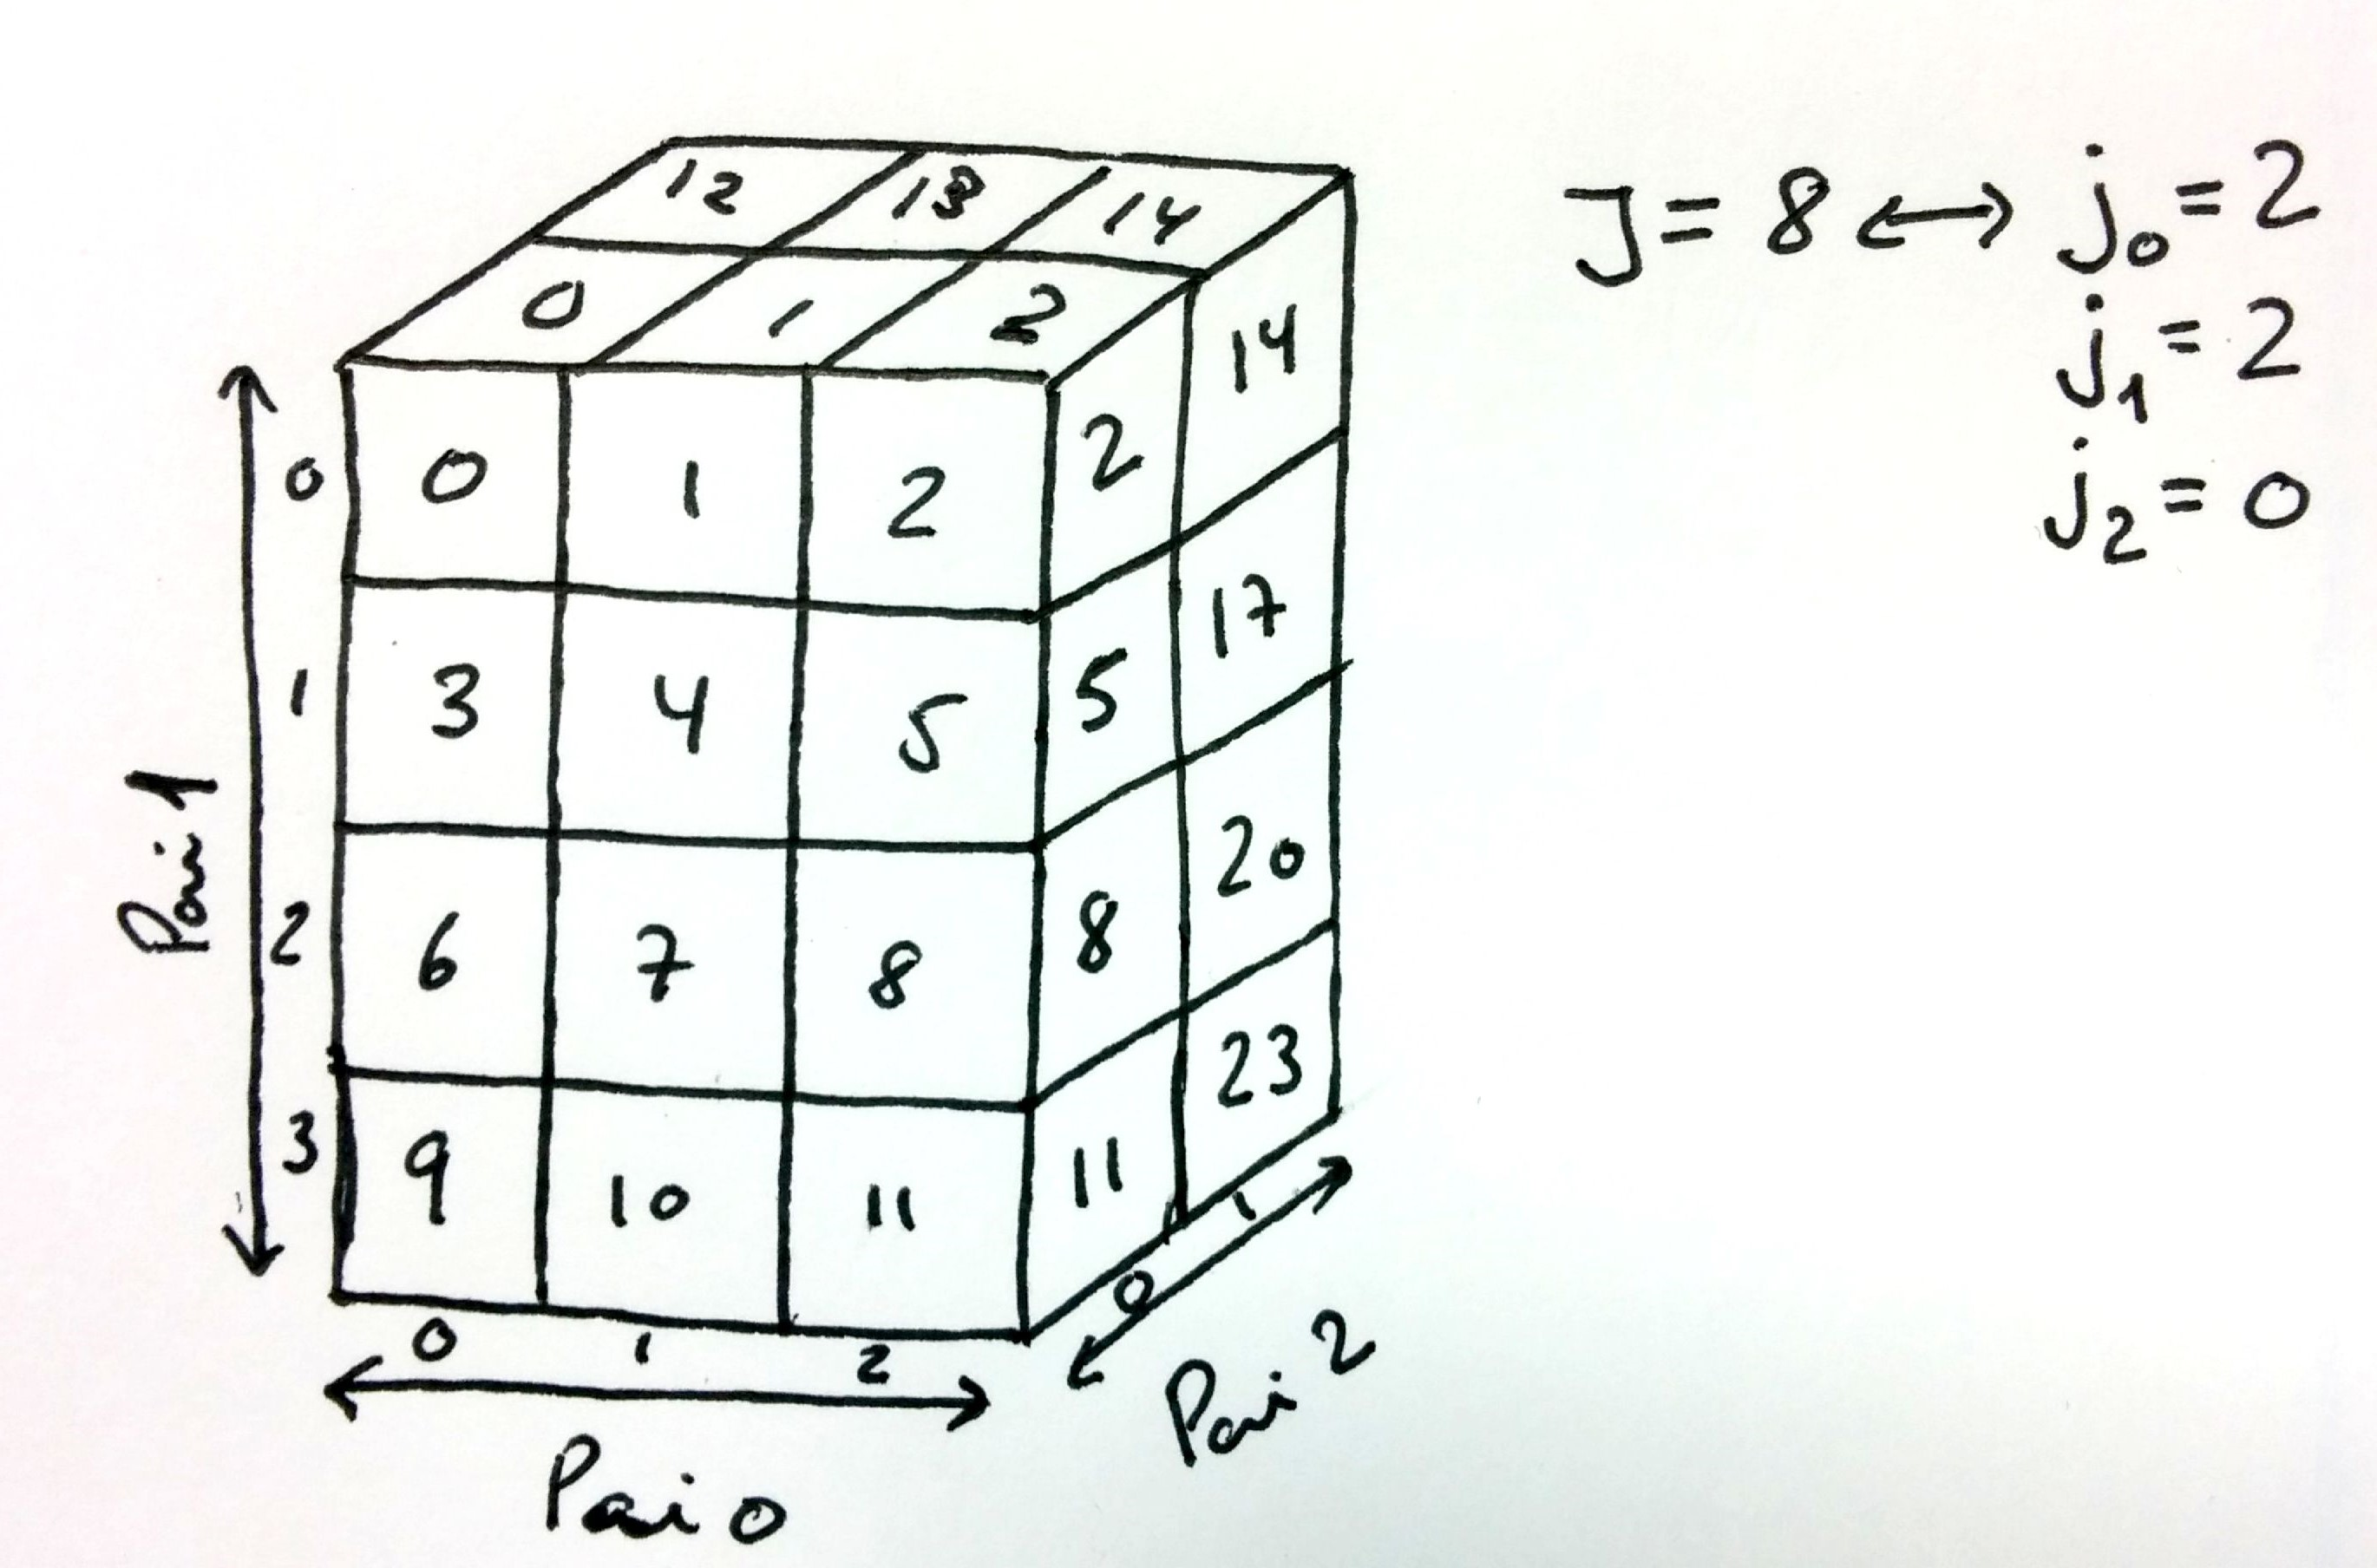
\includegraphics[keepaspectratio=true, scale=0.12]{./mapeamento}
	\caption{Representação visual do mapeamento.}
	\vspace{-0.8em}
\end{figure}

Na prática este método é implementado pelas seguintes parametrizações:

\begin{figure}[H]
	\centering
	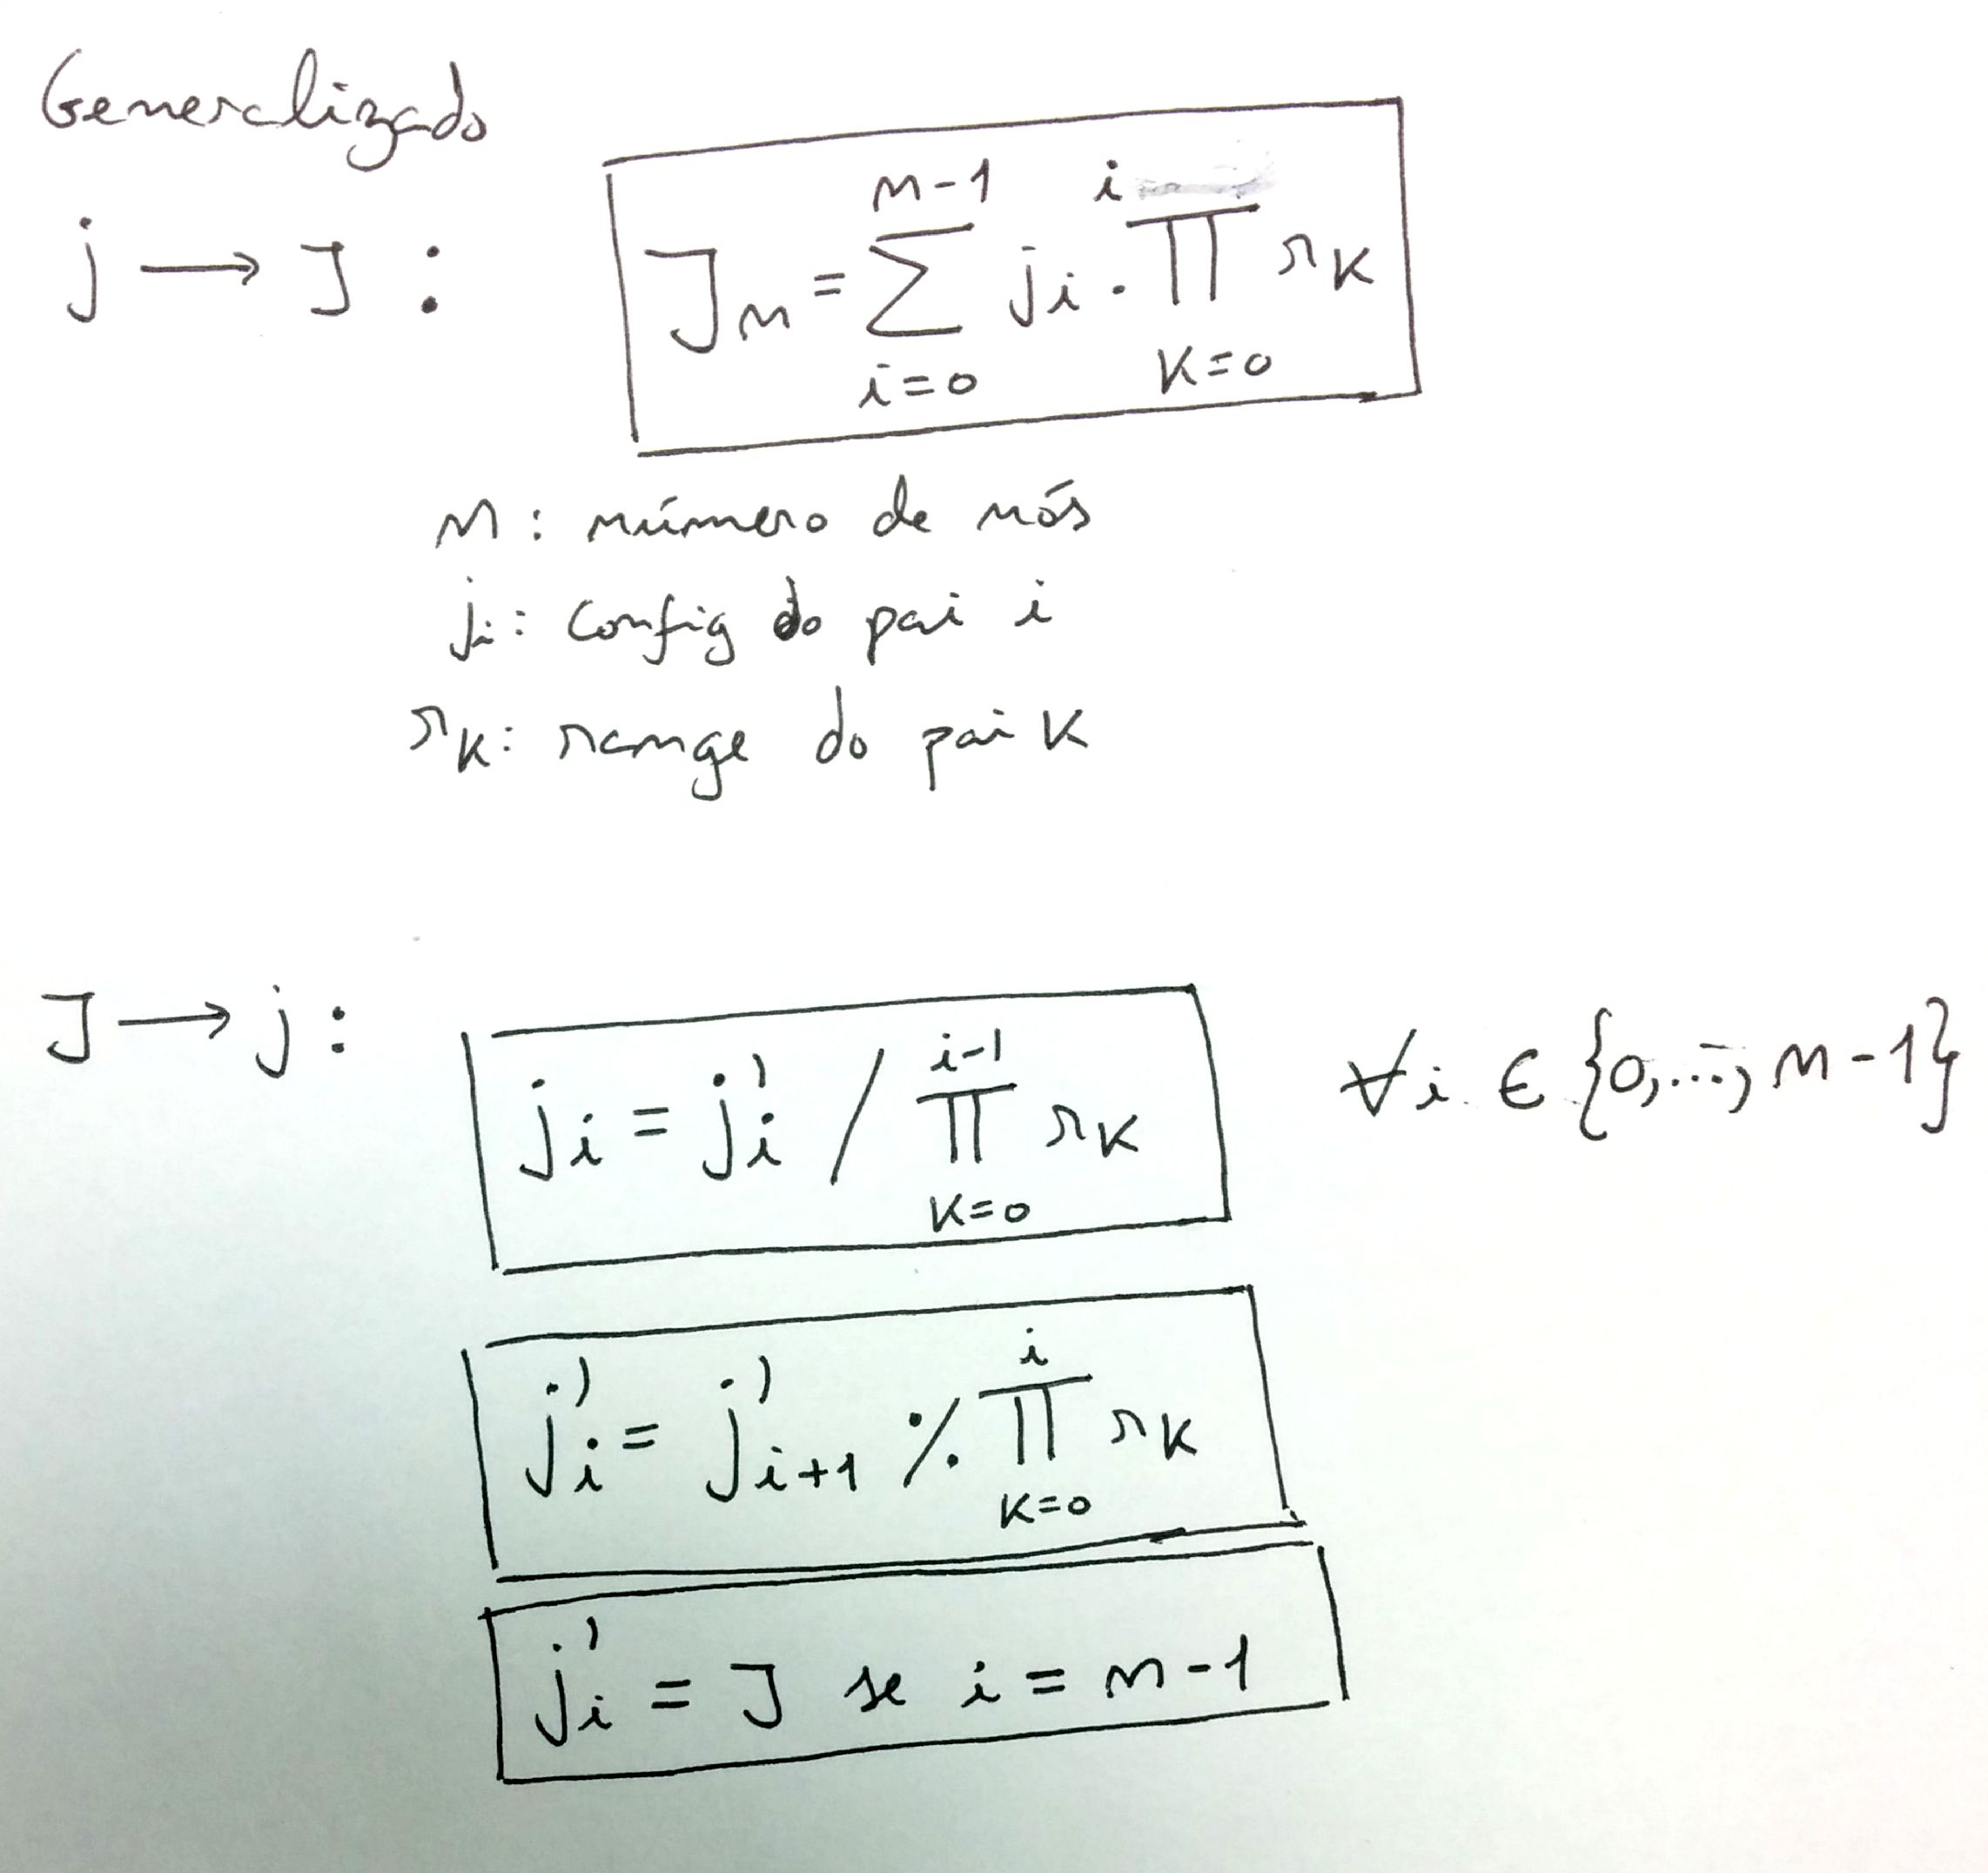
\includegraphics[keepaspectratio=true, scale=0.12]{./parametrizacoes}
	\caption{Parametrizações do mapeamento.}
	\vspace{-0.8em}
\end{figure}

\subsection{Critérios de paragem, recomeço e máximo}


\subsection{Operações de arestas}



\todo{explicar como se faz com as contagens, etc}

Durante a execuçao do algoritmo sao feitas operacoes sobre um grafo base e sao calculados os scores dos grafos resultantes. De forma a evitar cópia 

\subsection{\textit{Random-Restarts}}

Para se efectuar os \textit{random restarts} selecciona-se uma operaçao aleatoria atravès de um inteiro entre 0 e 1, sendo depois cada operaçao mapeada para: 0 corresponde a soma e 1 corresponde a remoçao.

\subsection{Tabu List}

A Tabu-List é implementada a partir de um HashSet do pacote java.util. Cada vez que se obtém um novo melhor score do grafo entre cada random-restart o grafo correspondente é clonado e armazenado na Tabu-List. A utilização desta estrutura de dados permite que a verificação da existência de um grafo seja feita o através do hashcode do grafo, o que garante um acesso muito rápido à tabu-list para verificar se um grafo gerado já foi percorrido. Esta garantia é importante, uma vez que esta operação é feita sempre que se gera um novo grafo.

\section{Testes Efectuados}
\subsection{Aprendizagem da DBN}

\subsubsection{Criação de DAGs}

Ao longo de toda a execução do programa é importante garantir que o grafo que representa a BN é um grafo acíclico. Para testar a implementação desta verificação criou-se um grafo inicial com três nós não ligados e, de seguida, efectuaram-se três operações de adição de arestas que resultariam num grafo com ciclos. 

As duas primeiras operações são realizadas com sucesso, mas a terceira, que iria gerar um ciclo nesse grafo, não chega a ser concluída, voltando o grafo ao seu estado de duas arestas apenas. 

\subsubsection{Mapeamento $j \leftrightarrow J$}

Outro aspecto importante da aprendizagem da DBN é o mapeamento de $j \leftrightarrow J$. Começou-se por testar esta operação isoladamente, ou seja, inicializou-se um \textit{array} correspondente aos \textit{ranges} dos pais, outro com os valores dos pais e outro ainda com o valor de $J$ que esses valores originariam. Uma vez verificado o correcto funcionamento do mapeamento este foi integrado no código do programa.

Face aos resultados obtidos para os testes explicados anteriormente assume-se que a aprendizagem da DBN está a funcionar.

\subsection{Inferências}

Inicialmente, para se verificar o funcionamento das inferências optou-se por verificar que a soma das probabilidades obtidas para os valores futuros possíveis da variável aleatória que se está a inferir dá próximo de 1, isto porque, obrigatoriamente, a variável aleatória toma no futuro um valor dos possíveis do seu \textit{range}. 

Este teste foi feito com recurso ao grafo da Figura \ref{fig:grafoforcado}, cuja criação se forçou na execução do programa.

\begin{figure}[H]
	\centering
	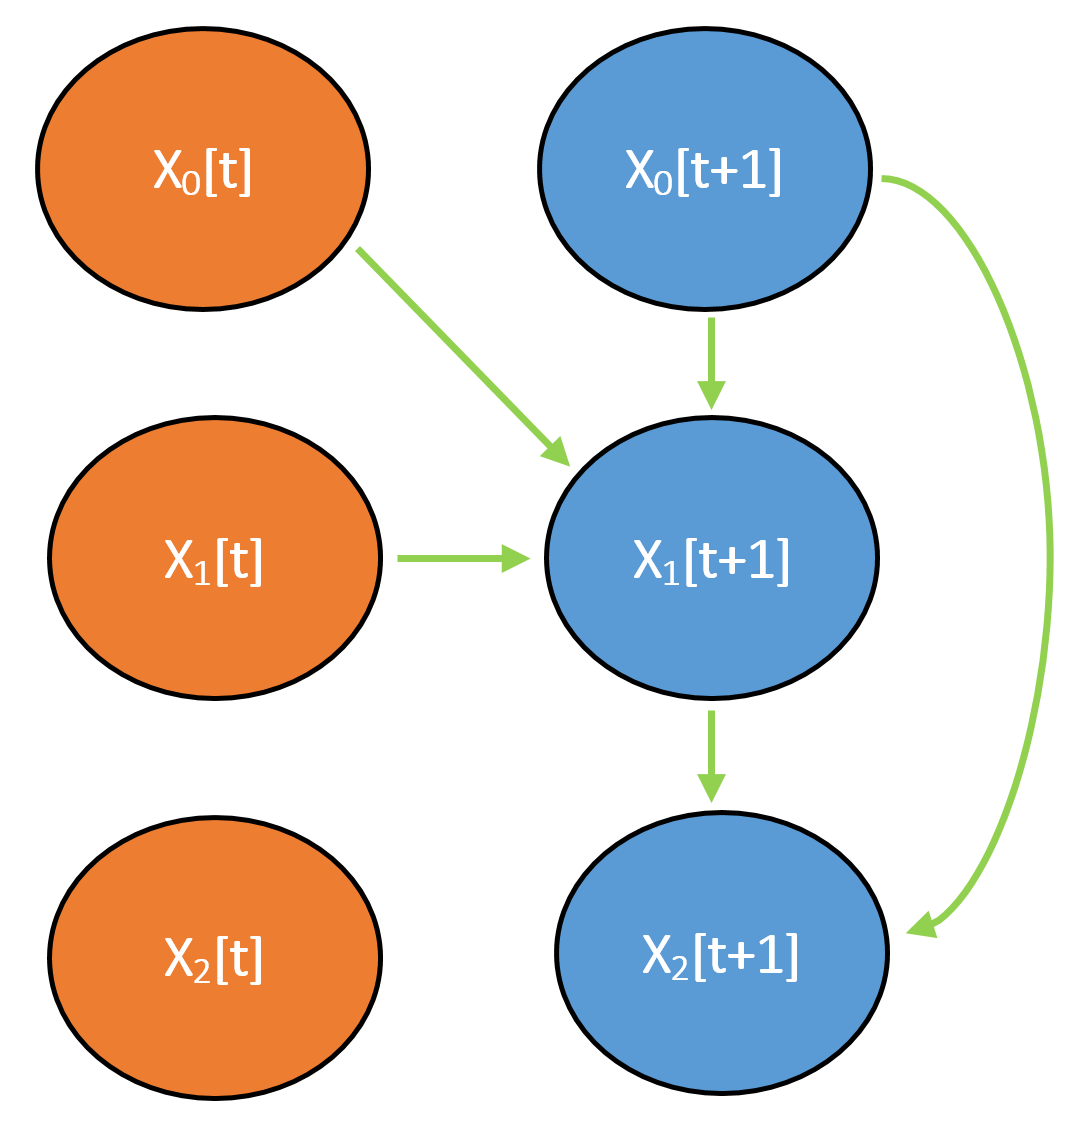
\includegraphics[keepaspectratio=true, scale=0.17]{teoricas/grafoforcado}
	\caption{Grafo da rede de transição utilizada para testar as inferências.}
	\vspace{-0.8em}
	\label{fig:grafoforcado}
\end{figure}

Assumindo todas as variáveis aleatórias como binárias, os valores obtidos para as probabilidades das três variáveis do futuro para os seus dois valores possíveis apresentam-se na seguinte tabela.

\begin{table}[H]
	\centering
	\caption{Probabilidades obtidas para os valores das variáveis aleatórias no futuro.}
	\vspace{-1.5mm}
	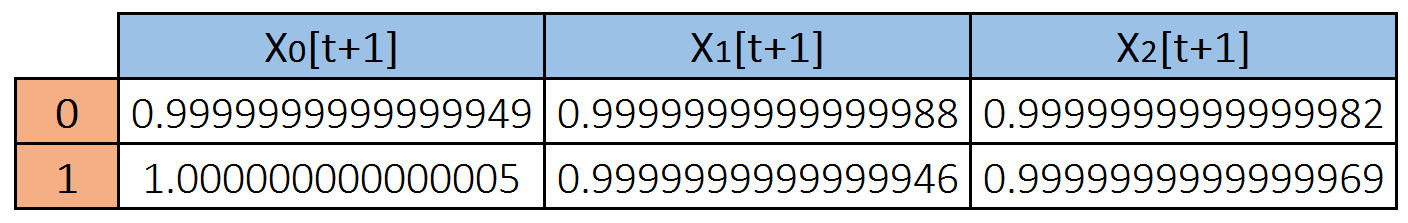
\includegraphics[keepaspectratio=true, scale=0.30]{tabelas/probabilidades}
\end{table}

\vspace{-1.5mm}
Como se pode ver, todas as probabilidades têm um valor muito próximo de 1, sendo normal que algumas sejam de facto maiores, uma vez que são calculadas com recurso a estimativas.

Para verificar as inferências que o programa obtém optou-se por usar o teste \#2 fornecido na página da cadeira como ficheiro de treino para se efectuar a aprendizagem da rede de Bayes. O ficheiro de teste construído corresponde aos valores do instante de tempo $t = 0$ do ficheiro de treino, sendo que, algumas das inferências, devem tomar valores próximos dos do instante de tempo $t = 1$ do ficheiro de treino:

\begin{lstlisting}
A, B, C, D, E, F, G
3, 3, 1, 0, 1, 1, 2
2, 3, 0, 3, 3, 1, 0
3, 1, 0, 1, 1, 2, 3
\end{lstlisting}

Considerando a construção da rede de Bayes sem \textit{random restarts} aquando da aplicação do algoritmo GHC tem-se a seguinte execução de programa para a inferência de todas as variáveis aleatórias. De notar que o teste apresentado de seguida foi executado no computador de um dos membros do grupo.

\begin{lstlisting}
Parameters: train-data-2.csv test-data-2-TRAIN.csv LL 0
Building DBN: 0.980114927 seconds
Initial network: 
=== Structure connectivity
A : C 
B : 
C : D 
D : G 
E : A 
F : A 
G : 
=== Scores
LL Score: -4.754887502163469
MDL Score: -131.55188755985597
Transition network: 
=== Inter-slice connectivity
A : G F 
B : G F 
C : F 
D : C G F 
E : F 
F : 
G : 
=== Intra-slice connectivity
A : C 
B : D 
C : D E 
D : 
E : B D 
F : G D E 
G : B A E 
=== Scores
LL Score: -4233.21662434474
MDL Score: -33449.233345448425
Performing inference:
-> instance 1: 
3, 3, 1, 0, 1, 1, 0
-> instance 2: 
2, 4, 0, 3, 1, 1, 0
-> instance 3: 
3, 2, 0, 2, 0, 1, 0
Infering with DBN: 9.704343301 seconds
\end{lstlisting}

Analisando os valores pretendidos e aqueles que foram de facto obtidos verifica-se uma eficácia de 61.91\%, um valor que se considera aceitável e, tendo em conta, que as somas das probabilidades já foram verificadas como estando próximas de 1 assume-se que as inferências estão correctas.

\subsection{\textit{Performance} Geral}

Relembrando o teste anterior que analisa as inferências com base no ficheiro de treino, efectuaram-se repetições desse teste ainda no mesmo computador mas com a inclusão de \textit{random restarts}.

De seguida apresenta-se o teste com o \textit{score} LL, com 10 \textit{random restarts} e com lista TABU.

\begin{lstlisting}
Parameters: train-data-2.csv test-data-2-TRAIN.csv LL 10
Building DBN: 1.6721379340000002 seconds
Initial network: 
=== Structure connectivity
A : C 
B : 
C : D 
D : G 
E : A 
F : A 
G : 
=== Scores
LL Score: -4.754887502163469
MDL Score: -131.55188755985597
Transition network: 
=== Inter-slice connectivity
A : G F 
B : G F 
C : F 
D : C G F 
E : F 
F : 
G : 
=== Intra-slice connectivity
A : C 
B : D 
C : D E 
D : 
E : B D 
F : G D E 
G : B A E 
=== Scores
LL Score: -4233.21662434474
MDL Score: -33449.233345448425
Performing inference:
-> instance 1: 
3, 3, 1, 0, 1, 1, 0
-> instance 2: 
2, 4, 0, 3, 1, 1, 0
-> instance 3: 
3, 2, 0, 2, 0, 1, 0
Infering with DBN: 8.963346173 seconds
\end{lstlisting}

O teste com 50 \textit{random restarts} apresenta-se em baixo.

\begin{lstlisting}
Parameters: train-data-2.csv test-data-2-TRAIN.csv LL 50
Building DBN: 5.8446849190000005 seconds
Initial network: 
=== Structure connectivity
A : C B D 
B : C D 
C : E F 
D : C F 
E : F 
F : 
G : A E F 
=== Scores
LL Score: -4.754887502163468
MDL Score: -2172.1911072383446
Transition network: 
=== Inter-slice connectivity
A : G F 
B : G F 
C : F 
D : C G F 
E : F 
F : 
G : 
=== Intra-slice connectivity
A : C 
B : D 
C : D E 
D : 
E : B D 
F : G D E 
G : B A E 
=== Scores
LL Score: -4233.21662434474
MDL Score: -33449.233345448425
Performing inference:
-> instance 1: 
3, 3, 1, 0, 1, 1, 0
-> instance 2: 
2, 4, 0, 3, 1, 1, 0
-> instance 3: 
3, 2, 0, 2, 0, 1, 0
Infering with DBN: 11.182559229 seconds
\end{lstlisting}

Como se pode ver, quantos mais \textit{random restarts} houver, mais tempo se demora na aprendizagem da BN, tal como expectável. No entanto, verifica-se que o \textit{score} obtido para a rede de transição não mudou, isto porque para se notarem diferenças é necessário ter pelo menos 500 ou 1000 \textit{random restarts}.

Assim, optou-se por gerar uma série de teste com valores diferentes de \textit{random restarts}, gerando gráficos dos \textit{scores} obtidos.

\begin{figure}[H]
	\centering
	\includegraphics[keepaspectratio=true, scale=0.17]{tabelas/testes}
	\caption{Testes efectuados ao programa.}
	\vspace{-0.8em}
\end{figure}

\todo{graficos do excel}


\section{Conclusão}

\end{document}